\chapter{Backend SDK}

Appsemble werkt met extensions, individueel ontwikkelde componenten, om een app te maken. Extensions worden ontwikkeld door d-centralize zelf en hopelijk in de toekomst door externe ontwikkelaars buiten het bedrijf. \\

Dit moet echter allemaal weergegeven worden. De ontwikkelaar moet namelijk complete vrijheid hebben om een extension te ontwikkelen met de tools die hij/zij wilt. Dit betekent dat er een ge{\"u}nificeerde oplossing moet zijn voor het laden van extensions. \\ 

In Appsemble wordt dit geregeld met iframes. Dit is een html element waarin een nieuwe webpagina geladen word. Ontwikkelaars moeten een extension dan ook eerst registreren bij de Appsemble API. Vanaf dit punt verschijnt het in de lijst met componenten. \\

Dit zorgt er echter voor dat een developer arbitrair scripts kan injecteren. Het is dus een veiligheidsrisico om developers te laten doen wat zij willen. Hier komt de SDK langs. \\

De SDK verzorgt een middenlaag tussen de extension en de verschillende services die zij willen gebruiken.Dit zorgt ervoor dat de extensions zelf goed beschermd zijn tegen boosdoeners, zonder dat er verminderde functionaliteit is.

\section{Requirements}

Om te zorgen dat er ontwikkeld kan worden voor Appsemble moet de backend van de SDK netjes ontwikkeld worden. Na discussie met collega's en de hoofddeveloper, zijn de volgende requirements eruit gekomen.

\begin{itemize}
	\item Kan API calls afhandelen
	\item Werkt met promises
	\item Kan specifieke functies aanroepen
	\item Is makkelijk uit te breiden
\end{itemize}

Om ervoor te zorgen dat er verschillende functies aangeroepen kunnen worden is er gebruikt gemaakt van een call-register. Dit is een map die een naam verbind aan een functie\footnote{In javascript zijn functies first-class citizen's en kunnen dus doorgegeven worden aan andere functies}\cite{stack1}. \\

Dit zorgt ervoor dat, indien de goede naam is gebruikt, de correcte functie zal worden uitgevoerd. Bij een functie call word dan ook een payload meegegeven. Dit is de data die een functie nodig uit te voeren. In feite is zijn het de functieparameters, maar dan verpakt in een javascript object. \\

Functies in de SDK worden samengevoegd in klassen, met betrekking tot hun doel. Dit zorgt ervoor dat dezelfde API's altijd in dezelfde klassen zitten. \\

Uiteindelijk worden deze klassen samengevoegd in de SDK, waarbij de SDK aan iedere klasse vraagt welke functies zij aanbieden. Dit word gecombineerd in een groot register, die vervolgens gebruikt wordt voor het aanroepen van zijnde functies. \\

De API's van de SDK kunnen alles wat mogelijk is binnen angular2, zoals het aanroepen van externe API's en het veranderen van de staat van Appsemble zelf\footnote{Mits hier een functie voor is}. \\

\subsection{Andere implementaties}

Voor een simpele versie van de API is overwogen om een vastgeprogrammeerd iets neer te zetten. Dit zou ervoor zorgen dat de API een stuk sneller af zou zijn, ten koste van de onderhoudbaarheid en uitbreidbaarheid. Uiteindelijk is er echter de keuze gemaakt om de API van de grond af uitbreidbaar te schrijven. Dit betekent dat er bijna geen vastgeprogrammeerde stukken code inzitten. \\

De andere optie was om te werken met reflectie voor het maken van een API. Dit is de meest uitbreidbare methode maar vergt echter een stuk meer werk om gedaan te krijgen. Daarom is gekozen voor de meest efficiente qua tijd en complexiteit, waar modules zichzelf registreren bij de SDK om vervolgens aangeroepen te worden.

\begin{figure}
	\centering
	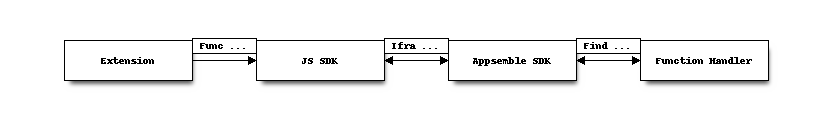
\includegraphics[width=\linewidth]{../dcentralize-diagrams/seq/sdk-call}
	\caption{\textit{Sequence Diagram van een SDK call}}
	\label{fig:SDK-call}
\end{figure}

\section{Geschreven SDK componenten}

\subsection{Resources}

De resources API biedt de mogelijkheid voor developers om data te lezen en te schrijven. Het word gebackt door de google cloud database. Ontwikkelaars kunnen door middel van resource configurations zelf een tabel aanmaken in deze database. Vervolgens kan met een simpele SDK call hier data naar geschreven worden.

\subsection{Appsemble integratie}

De Appsemble API biedt toegang tot interne functionaliteit van Appsemble. Deze kan worden gebruikt voor bepaalde acties van Appsemble zelf te starten, zoals het navigatie menu openen of toegang aanvragen tot de huidige metadata van de app.

\subsection{Files}

De Files API zorgt voor het werken met bestanden en het lezen van IO streams. Zo kan met de File API bijvoorbeeld een bestand van het systeem geselecteerd worden om in te lezen of kan een foto gemaakt worden. \\

Deze API verzorgt ook functionaliteit om ervoor te zorgen dat alle bestanden die in en uit gaan van hetzelfde formaat zijn\footnote{Appsemble gebruik Blob's in tegenstelling tot een base64-encoded url}. Deze standaard is besloten door het Appsemble team.